\documentclass[11pt]{article}
\usepackage{amsmath, amssymb}
\usepackage{geometry}
\usepackage{hyperref}
\usepackage{graphicx}
\usepackage{booktabs}
\geometry{margin=2.5cm}
\emergencystretch=2em

\newcommand{\ket}[1]{|#1\rangle}
\newcommand{\bra}[1]{\langle#1|}
\newcommand{\Oedge}{X_0 Z_1\cdots Z_{L-2} X_{L-1}}
\newcommand{\Tr}{\operatorname{Tr}}

\title{Week 9 Notes: Circuit-Level Gate Noise on the VQE\\
\large Integration, Verification, and Depth Scaling}
\author{}
\date{\today}

\begin{document}
\maketitle

\section{Purpose and Context}

Week 7 produced a \emph{validated} parity-constrained VQE: across the chemical-potential sweep it returns optimal parameters $\theta^*(\mu)$ that reproduce the even-parity ground state, benchmarked against exact diagonalization for energy, parity, subspace fidelity, and the edge string $O_{\mathrm{edge}}=\Oedge$. Week 7 also ran a \emph{depth diagnostic}: \emph{noiselessly}, the subspace infidelity falls as the number of ansatz repetitions $r$ grows, so a deeper ansatz prepares a better state.

That conclusion is only half the story on real hardware. A NISQ device builds the state with a \emph{circuit}, and error enters \emph{through the gates}: every entangling operation injects a fresh error channel, so the total corruption grows with the gate count and the circuit depth. Week 9 integrates this correctly with Qiskit's noise stack and asks the quantitative question Week 7 could only hint at: as the ansatz deepens, the prepared state improves but the accumulated gate noise worsens --- so how does the edge-string diagnostic actually behave?

This note has three goals:
\begin{enumerate}
  \item \textbf{Theory.} Treat a noisy gate as a completely positive trace-preserving (CPTP) map composed with the ideal unitary, and write the depolarizing and thermal-relaxation channels in Kraus/Pauli form.
  \item \textbf{Practice.} Build a Qiskit \texttt{NoiseModel}, attach gate errors to instructions, read the edge string from a density-matrix simulation, and \textbf{verify} the integration against an independent exact gate-by-gate reference.
  \item \textbf{Result.} Quantify how the edge-string diagnostic scales with ansatz depth $r$ under per-CNOT noise --- the expressibility-versus-noise trade-off.
\end{enumerate}

All conventions follow the existing repository: the little-endian Jordan--Wigner qubit Hamiltonian and the edge string $O_{\mathrm{edge}}=\Oedge$ from \texttt{block3\_core.py}.

\section{Gate Errors as Quantum Channels (Theory)}

\subsection{The gate-then-error model}

An ideal gate acts by unitary conjugation, $\mathcal{U}_g(\rho)=U_g\,\rho\,U_g^\dagger$. A noisy gate is the ideal unitary followed by an error channel $\mathcal{E}_g$,
\[
  \tilde{\mathcal{U}}_g=\mathcal{E}_g\circ\mathcal{U}_g ,
\qquad
  \mathcal{E}_g(\rho)=\sum_k K_k\,\rho\,K_k^\dagger ,
\qquad
  \sum_k K_k^\dagger K_k = I ,
\]
where the completeness relation guarantees the map is CPTP. This is exactly the model Qiskit Aer implements: for every instruction in the \emph{transpiled} circuit, the associated error channel is applied immediately after that instruction. For a circuit $U=U_{g_M}\cdots U_{g_1}$,
\[
  \rho_{\mathrm{out}}
  =\bigl(\mathcal{E}_{g_M}\circ\mathcal{U}_{g_M}\bigr)\circ\cdots\circ
   \bigl(\mathcal{E}_{g_1}\circ\mathcal{U}_{g_1}\bigr)(\rho_{\mathrm{in}}).
\]
The central consequence is that \textbf{noise scales with gate count and depth}: a deeper circuit composes more error channels.

\subsection{Physical origin: from Lindblad to Pauli channels}

These channels are not arbitrary. A Markovian open system obeys the Lindblad equation
\[
  \dot{\rho}=-i[H,\rho]+\sum_k\Bigl(L_k\rho L_k^\dagger-\tfrac12\{L_k^\dagger L_k,\rho\}\Bigr),
\]
and integrating over a finite gate duration $\tau$ produces a CPTP (Kraus) map. Isotropic, fully symmetric noise integrates to the \emph{depolarizing} channel; energy relaxation $\ket{1}\to\ket{0}$ to \emph{amplitude damping} ($T_1$); pure loss of phase coherence to \emph{phase damping} ($T_2$). The practical Qiskit channels below are the gate-duration-integrated shadows of physical decoherence.

\section{The Depolarizing Channel}

The $n$-qubit depolarizing channel mixes the state toward the maximally mixed state. Qiskit's \texttt{depolarizing\_error(p, n)} uses the ``with probability $p$, replace by the maximally mixed state'' convention,
\[
  \mathcal{E}^{\mathrm{dep}}_p(\rho)
  =(1-p)\,\rho+p\,\frac{\Tr\rho}{2^n}\,I .
\]
Using the Pauli twirl identity $\frac{1}{4^n}\sum_{P}P\rho P^\dagger=\frac{\Tr\rho}{2^n}I$ (sum over all $4^n$ Pauli strings), this is equivalently a random-Pauli channel,
\[
  \mathcal{E}^{\mathrm{dep}}_p(\rho)
  =\Bigl(1-p\,\tfrac{4^n-1}{4^n}\Bigr)\rho
   +\frac{p}{4^n}\sum_{P\neq I}P\rho P^\dagger .
\]
We attach a two-qubit depolarizing error of strength $p_{\mathrm{cx}}$ after every \texttt{cx}, the dominant error on superconducting hardware.

\section{Thermal Relaxation as a Gate Error ($T_1$/$T_2$)}

Depolarizing noise is symmetric and structureless --- the right first check, but not the real physics. The realistic upgrade attaches a \emph{thermal relaxation} channel that depends on the gate duration $\tau$ and the device coherence times. Qiskit provides \texttt{thermal\_relaxation\_error(t1, t2, time)}, combining:
\begin{itemize}
  \item \textbf{Amplitude damping} ($T_1$): excitation-loss probability $p_{T_1}=1-e^{-\tau/T_1}$, mapping $\ket{1}\to\ket{0}$;
  \item \textbf{Phase damping} ($T_2$): loss of off-diagonal coherence at rate set by $T_2$, with physical consistency $T_2\le 2T_1$ (Qiskit enforces this).
\end{itemize}

\paragraph{Why this matters for the Majorana diagnostic.} Two effects are qualitatively distinct from symmetric depolarizing contrast loss:
\begin{itemize}
  \item \textbf{$T_1$ is parity poisoning.} In the Jordan--Wigner encoding qubit occupation tracks fermion occupation, so $\ket{1}\to\ket{0}$ flips the fermion parity and pushes the state out of the even sector the diagnostic lives in.
  \item \textbf{$T_2$ kills non-local coherence.} The edge string is an endpoint-to-endpoint correlator; pure dephasing suppresses exactly the off-diagonal coherence that carries it.
\end{itemize}
Because relaxation is gate-duration-dependent and two-qubit gates are the longest, putting the dominant noise on the \texttt{cx} operations is justified from first principles.

\section{Building and Verifying a NoiseModel (Practice)}

\subsection{Construct, attach, read out}

\begin{verbatim}
from qiskit import transpile
from qiskit.quantum_info import SparsePauliOp
from qiskit_aer import AerSimulator
from qiskit_aer.noise import (NoiseModel, depolarizing_error,
                              thermal_relaxation_error)

nm = NoiseModel()
nm.add_all_qubit_quantum_error(depolarizing_error(p_cx, 2), ['cx'])

sim = AerSimulator(method='density_matrix', noise_model=nm)
qc = ansatz.assign_parameters(theta).copy()     # the Week 7 VQE state prep
qc.save_density_matrix()
rho = sim.run(transpile(qc, sim)).result().data()['density_matrix']

O_edge = SparsePauliOp(['XZZX'], [1.0])          # L = 4 edge string
s = float(rho.expectation_value(O_edge).real)
\end{verbatim}
\texttt{add\_all\_qubit\_quantum\_error} applies the channel after \emph{every} occurrence of the named gate.

\paragraph{The transpilation gotcha.} Errors attach to gate \emph{names}, and a noise model only fires on names that survive transpilation into the simulator basis. We transpile everything to a fixed basis \texttt{['rz','sx','cx']} (\texttt{block4.py}, \texttt{BASIS\_GATES}) so the \texttt{cx} the error is attached to is exactly the \texttt{cx} the circuit runs. If the target basis used \texttt{ecr} or \texttt{cz}, an error attached to \texttt{cx} would never trigger.

\subsection{Precise verification: an independent exact reference}

To prove the gate noise is integrated correctly --- not just plausibly --- we reproduce the noisy circuit a second, independent way and compare. The function \texttt{exact\_reference\_edge} in \texttt{block4.py} transpiles the same circuit, then evolves the density matrix \emph{by hand}, gate by gate: it applies each gate's unitary as a \texttt{quantum\_info.Operator} and, after every \texttt{cx}, applies the two-qubit depolarizing channel as a \texttt{SuperOp}. This uses none of the Aer simulator's noise machinery, so agreement is a genuine cross-check.

\begin{verbatim}
from qiskit.quantum_info import DensityMatrix, Operator, SuperOp

dep = SuperOp(depolarizing_error(p_cx, 2))
dm = DensityMatrix.from_label('0' * L)
for inst in transpile(qc, basis_gates=['rz','sx','cx'], optimization_level=0).data:
    qargs = [qc.find_bit(q).index for q in inst.qubits]
    dm = dm.evolve(Operator(inst.operation), qargs=qargs)
    if inst.operation.name == 'cx':
        dm = dm.evolve(dep, qargs=qargs)
\end{verbatim}

Run across the whole $\mu$ sweep, the Aer \texttt{NoiseModel} edge string and this exact reference agree to $\max|\,\cdot\,|\sim10^{-15}$ at every $\mu$ (Fig.~\ref{fig:verify}, left). The gate error is therefore correctly integrated over the entire diagnostic, not merely at one density matrix.

\section{Noise Integrated Through the Gates, by reps}

This is the central result. The linear-entanglement \texttt{EfficientSU2} ansatz at depth $r$ contains
\[
  \#\,\mathrm{CNOTs}=r\,(L-1),
\]
and each carries a depolarizing channel. The measured edge string is therefore a product of two opposing factors,
\begin{equation}
  |\langle O_{\mathrm{edge}}\rangle|_{\mathrm{meas}}(r)
  \;\approx\;
  \underbrace{|\langle O_{\mathrm{edge}}\rangle|_{\mathrm{ideal}}(r)}_{\text{expressibility, rises with }r}
  \;\times\;
  \underbrace{(1-p_{\mathrm{cx}})^{\,r(L-1)}}_{\text{gate noise, falls with }r}.
  \label{eq:tradeoff}
\end{equation}
Week 7 established that the first factor rises toward $1$ with depth (lower infidelity); Eq.~\eqref{eq:tradeoff} shows the second factor falls exponentially in depth. Their product is non-monotonic, so there is an \textbf{optimal ansatz depth} on a noisy device --- the precise statement of the expressibility-versus-noise trade-off.

Plot~2 of \texttt{block4.py} makes this concrete (Fig.~\ref{fig:depth}). For each depth $r$ it prepares the VQE state across $\mu$ at fixed per-\texttt{cx} strength $p_{\mathrm{cx}}$, so the only thing changing between curves is the CNOT count $r(L-1)$. As $r$ grows, the measured edge-string sweep is pushed down and the topological/trivial contrast flattens: the same circuit depth that buys a better noiseless state costs measurable signal once the gates are noisy. An independent pure-numpy gate-by-gate evolution reproduces the same monotonic decay of purity and edge-string magnitude with CNOT count, confirming the mechanism is the accumulated channel and not a simulator artifact.

\begin{figure}[h]
  \centering
  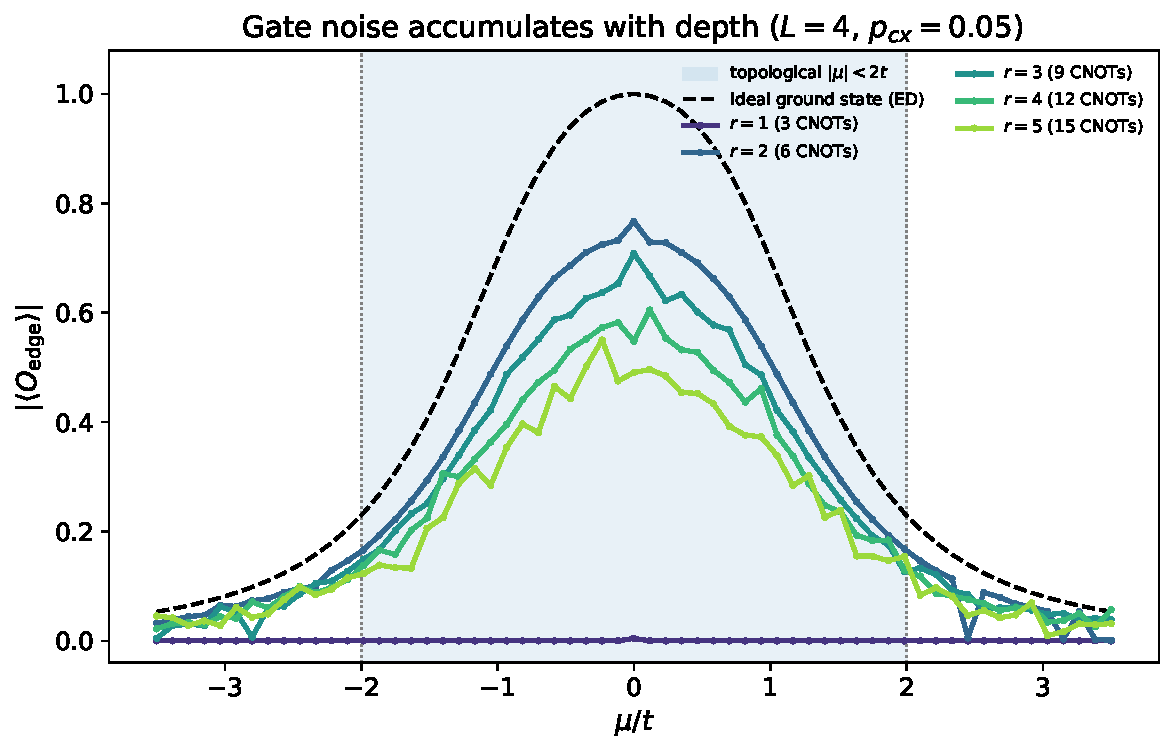
\includegraphics[width=0.9\linewidth]{../plots/block4_week9_depth_sweep.pdf}
  \caption{Edge-string sweep at increasing ansatz depth $r$ under a fixed per-\texttt{cx} depolarizing strength. The noiseless curve (dashed) marks the topological plateau $|\mu|<2t$; as the circuit deepens, $r(L-1)$ noisy CNOTs push the measured diagnostic down and flatten the phase contrast.}
  \label{fig:depth}
\end{figure}

\section{Verification and the Thermal Model}

Plot~3 of \texttt{block4.py} combines the precise verification with the realistic noise upgrade (Fig.~\ref{fig:verify}). The left panel is the exact-versus-Aer cross-check across $\mu$ described above, agreeing to $\sim10^{-15}$. The right panel keeps the same VQE states but swaps the depolarizing channel for \texttt{thermal\_relaxation\_error}$(T_1,T_2,\tau)$ on each \texttt{cx}, with device-realistic coherence times $T_1=80\,\mu$s, $T_2=60\,\mu$s and a $\tau=300$\,ns gate. At these parameters the per-gate relaxation error is only $1-e^{-\tau/T_1}\approx0.4\%$, far below the deliberately large $p_{\mathrm{cx}}=0.10$ depolarizing strength, so the thermal curve sits much closer to the ideal: realistic relaxation is the \emph{subdominant} channel on a shallow circuit, consistent with depolarizing/readout being the first bottlenecks. The thermal channel nonetheless differs in \emph{kind} rather than only magnitude --- $T_1$ leaks the state out of the even-parity sector (parity poisoning) and $T_2$ attacks exactly the endpoint coherence the non-local string depends on --- which is why it is the physically correct model to carry forward even when its present-parameter effect is mild.

\begin{figure}[h]
  \centering
  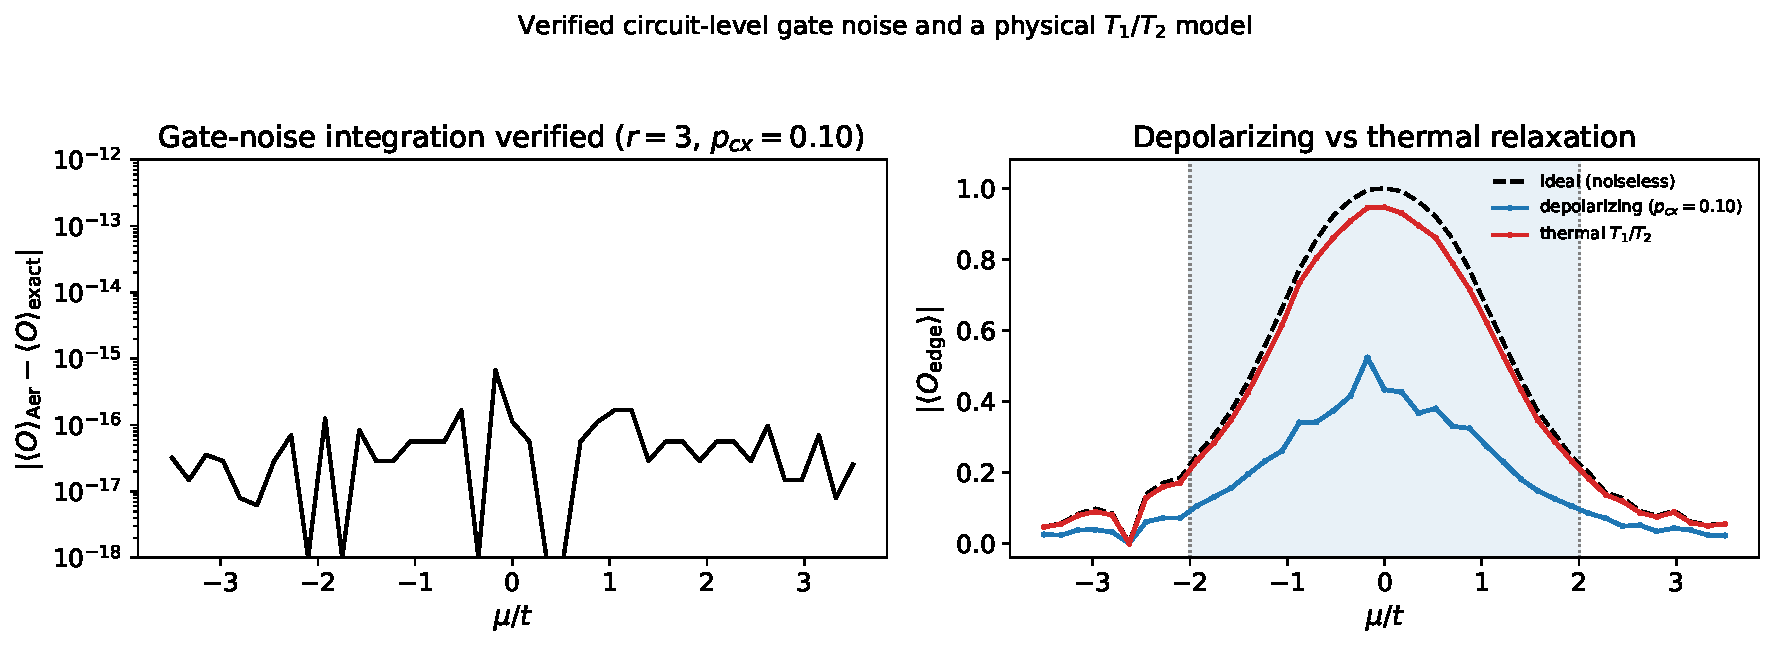
\includegraphics[width=0.98\linewidth]{../plots/block4_week9_verification.pdf}
  \caption{Left: the Aer \texttt{NoiseModel} edge string and the independent exact gate-by-gate reference agree to $\sim10^{-15}$ across the whole $\mu$ sweep, verifying the gate-error integration. Right: depolarizing versus a physical $T_1/T_2$ thermal-relaxation channel at matched gate placement; the thermal model is the realistic upgrade.}
  \label{fig:verify}
\end{figure}

\section{Connection to the Majorana Edge-String Diagnostic}

The edge string is the most exposed observable in the whole program because it is non-local: its value is a coherent correlation built across the chain by a ladder of two-qubit gates. In the circuit-level model every noisy \texttt{cx} injects depolarization that pulls the endpoint-to-endpoint coherence toward zero, suppressing $|\langle O_{\mathrm{edge}}\rangle|$ even when local observables still look reasonable; $T_1$ relaxation additionally poisons the parity sector, which is qualitatively worse than contrast loss; and the transition regions near $|\mu|\approx2t$ are the most fragile, since the ideal signal is already changing rapidly there and little noise blurs the apparent phase boundary.

\section{What This Enables Next}

With gate errors integrated and verified at the circuit level, the next steps are concrete:
\begin{itemize}
  \item \textbf{Noisy VQE optimization.} Optimize with a \texttt{NoiseModel}-backed Aer \texttt{Estimator}, so every cost evaluation is corrupted and the optimizer must search through noise rather than receiving a frozen validated state.
  \item \textbf{Backend-calibrated noise.} Use \texttt{NoiseModel.from\_backend(...)} for real device $T_1$/$T_2$ and gate-error data.
  \item \textbf{The professor's questions.} With a faithful noisy-VQE pipeline in place, return to whether the parity is protected by topology and how the chain length interacts with the depth trade-off found here.
\end{itemize}

\end{document}
